\documentclass[11pt]{article}

\usepackage[T1]{fontenc}
\usepackage[utf8]{inputenc}
\usepackage{lmodern}
\usepackage{amsmath,amssymb,amsthm,mathtools}
\usepackage{microtype}
\usepackage{booktabs}
\usepackage{enumitem}
\usepackage{tabularx}
\usepackage{needspace}
\usepackage{array}
\usepackage[margin=1in,top=0.9in,bottom=1in]{geometry}
\usepackage{fancyhdr}
\usepackage{lastpage}
\usepackage{tikz}
\usepackage[hidelinks]{hyperref}

\pagestyle{fancy}
\fancyhf{}
\lhead{\small BIO 2970 --- Selection Practice Exam S2}
\rhead{\small Name: \underline{\hspace{5cm}}}
\cfoot{\small\thepage\ of \pageref*{LastPage}}
\renewcommand{\headrulewidth}{0.4pt}
\setlength{\headheight}{14pt}

% answer text, for KEY documents only
\newcommand{\keyans}[1]{\par\medskip\noindent\textit{Answer.}\ #1\par\medskip}
\newcommand{\work}[1]{\par\vspace{#1}}
\newcommand{\opt}[1]{\makebox[1.9em][l]{(#1)}}
\newcolumntype{Y}{>{\raggedright\arraybackslash}X}
\setlist[enumerate,1]{leftmargin=2em,labelsep=0.6em}
\hyphenpenalty=1000
\relpenalty=10000
\binoppenalty=10000
\begin{document}

\begin{center}
  {\LARGE\bfseries Natural Selection --- Practice Exam S2}\\[5pt]
  {\large Level 2 \quad\textbullet\quad Harder and multi-step}\\[6pt]
  BIO 2970 \quad\textbullet\quad Fitness and Selection, Lectures 23 and 24 \quad\textbullet\quad Fall 2026\\[3pt]
  \rule{\textwidth}{0.8pt}\\[3pt]
  {\small Raw counts, survival and fecundity together, the generation after selection, and which allele is \(p\).\\[2pt] 24 multiple-choice questions of equal weight. Choose the single best answer and mark it on the answer sheet on the second-to-last page. Calculator allowed. Give three decimals unless a question says otherwise.}
\end{center}
\vspace{0.4em}

\begin{enumerate}[label=\textbf{\arabic*.}, leftmargin=2em, itemsep=1.4em]
\needspace{9\baselineskip}
\item 100 zygotes are 40 AA, 40 Aa and 20 aa. Survivors to breeding are 30 AA, 24 Aa and 6 aa, and all survivors breed equally. What is \(\Delta q\) for a?
\par\smallskip\noindent\begin{tabularx}{\linewidth}{@{}YYYY@{}}
\makebox[1.9em][l]{(A)}\(-\)0.083 & \makebox[1.9em][l]{(B)}+0.100 & \makebox[1.9em][l]{(C)}\(-\)0.100 & \makebox[1.9em][l]{(D)}\(-\)0.300 \\
\end{tabularx}
\work{1.6cm}
\needspace{9\baselineskip}
\item In that population, what is \(\overline{W}\) and what does it mean physically?
\par\smallskip
\begin{enumerate}[label={}, leftmargin=2.4em, labelwidth=0pt, itemsep=2pt, topsep=0pt]
\item \hspace*{-2.4em}\makebox[2.4em][l]{(A)}0.55, the average of the three survivorships
\item \hspace*{-2.4em}\makebox[2.4em][l]{(B)}0.60, the fraction of zygotes that survived
\item \hspace*{-2.4em}\makebox[2.4em][l]{(C)}0.60, the frequency of A
\item \hspace*{-2.4em}\makebox[2.4em][l]{(D)}1.00, because survivors all breed
\end{enumerate}
\needspace{9\baselineskip}
\item Hardy-Weinberg, \(q\) = 0.5. Viability is 0.9, 0.8 and 0.5 and fecundity is 2, 3 and 4 for AA, Aa and aa. What is \(q\) after selection?
\par\smallskip\noindent\begin{tabularx}{\linewidth}{@{}YYYY@{}}
\makebox[1.9em][l]{(A)}0.500 & \makebox[1.9em][l]{(B)}0.433 & \makebox[1.9em][l]{(C)}0.512 & \makebox[1.9em][l]{(D)}0.583 \\
\end{tabularx}
\work{1.6cm}
\needspace{9\baselineskip}
\item Hardy-Weinberg, \(q\) = 0.4, \(W\) = 0.9, 1 and 0.6 for AA, Aa and aa. What is the Aa frequency among the survivors, right after selection?
\par\smallskip\noindent\begin{tabularx}{\linewidth}{@{}YYYY@{}}
\makebox[1.9em][l]{(A)}0.480 & \makebox[1.9em][l]{(B)}0.468 & \makebox[1.9em][l]{(C)}0.533 & \makebox[1.9em][l]{(D)}0.267 \\
\end{tabularx}
\work{1.6cm}
\needspace{9\baselineskip}
\item Same population. What is the mean fitness of the next generation, after the survivors mate at random?
\par\smallskip\noindent\begin{tabularx}{\linewidth}{@{}YYYY@{}}
\makebox[1.9em][l]{(A)}0.921 & \makebox[1.9em][l]{(B)}1.000 & \makebox[1.9em][l]{(C)}0.900 & \makebox[1.9em][l]{(D)}0.905 \\
\end{tabularx}
\needspace{9\baselineskip}
\item Same population, \(q\) = 0.4, \(\overline{W}\) = 0.900. Using the average excess of A, what is \(\Delta p\)?
\par\smallskip\noindent\begin{tabularx}{\linewidth}{@{}YYYY@{}}
\makebox[1.9em][l]{(A)}\(-\)0.027 & \makebox[1.9em][l]{(B)}+0.040 & \makebox[1.9em][l]{(C)}+0.027 & \makebox[1.9em][l]{(D)}+0.018 \\
\end{tabularx}
\work{1.6cm}
\needspace{9\baselineskip}
\item Can an allele that kills every homozygote have a positive average excess?
\par\smallskip
\begin{enumerate}[label={}, leftmargin=2.4em, labelwidth=0pt, itemsep=2pt, topsep=0pt]
\item \hspace*{-2.4em}\makebox[2.4em][l]{(A)}Yes, if it is rare and the heterozygote is fitter than the population average
\item \hspace*{-2.4em}\makebox[2.4em][l]{(B)}Only if it is dominant
\item \hspace*{-2.4em}\makebox[2.4em][l]{(C)}Only if the population is not in Hardy-Weinberg
\item \hspace*{-2.4em}\makebox[2.4em][l]{(D)}No, a lethal allele always has negative average excess
\end{enumerate}
\needspace{9\baselineskip}
\item Absolute fitnesses are 2.4, 1.6 and 1.6 for BB, Bb and bb. Which model applies, and which allele is \(q\)?
\par\smallskip
\begin{enumerate}[label={}, leftmargin=2.4em, labelwidth=0pt, itemsep=2pt, topsep=0pt]
\item \hspace*{-2.4em}\makebox[2.4em][l]{(A)}Selection against the dominant, \(q\) = b
\item \hspace*{-2.4em}\makebox[2.4em][l]{(B)}Selection against the recessive, \(q\) = b
\item \hspace*{-2.4em}\makebox[2.4em][l]{(C)}Selection against the recessive, \(q\) = B
\item \hspace*{-2.4em}\makebox[2.4em][l]{(D)}Selection against the dominant, \(q\) = B
\end{enumerate}
\needspace{9\baselineskip}
\item Selection against the recessive with \(s\) = 0.6 and \(q\) = 0.5. What is \(\Delta q\)?
\par\smallskip\noindent\begin{tabularx}{\linewidth}{@{}YYYY@{}}
\makebox[1.9em][l]{(A)}\(-\)0.150 & \makebox[1.9em][l]{(B)}\(-\)0.136 & \makebox[1.9em][l]{(C)}\(-\)0.088 & \makebox[1.9em][l]{(D)}\(-\)0.075 \\
\end{tabularx}
\work{1.6cm}
\needspace{9\baselineskip}
\item A harmful allele is at \(q\) = 0.02 with \(s\) = 0.5. Roughly how many times faster is it removed if it is dominant than if it is recessive?
\par\smallskip\noindent\begin{tabularx}{\linewidth}{@{}YY@{}}
\makebox[1.9em][l]{(A)}About the same & \makebox[1.9em][l]{(B)}About 50 times \\[3pt]
\makebox[1.9em][l]{(C)}About 2 times & \makebox[1.9em][l]{(D)}About 2{,}500 times \\
\end{tabularx}
\needspace{9\baselineskip}
\item A lethal recessive (\(s\) = 1) has \(q'\) = \(q\)/(1 + \(q\)) each generation, so 1/\(q\) rises by exactly 1 per generation. How many generations to go from \(q\) = 0.02 to 0.01?
\par\smallskip\noindent\begin{tabularx}{\linewidth}{@{}YYYY@{}}
\makebox[1.9em][l]{(A)}50 & \makebox[1.9em][l]{(B)}1 & \makebox[1.9em][l]{(C)}100 & \makebox[1.9em][l]{(D)}25 \\
\end{tabularx}
\work{1.6cm}
\needspace{9\baselineskip}
\item Relative fitnesses are 0.75, 1 and 0.5 for AA, Aa and aa. What is the equilibrium frequency of A?
\par\smallskip\noindent\begin{tabularx}{\linewidth}{@{}YYYY@{}}
\makebox[1.9em][l]{(A)}0.333 & \makebox[1.9em][l]{(B)}0.667 & \makebox[1.9em][l]{(C)}0.500 & \makebox[1.9em][l]{(D)}0.250 \\
\end{tabularx}
\work{1.6cm}
\needspace{9\baselineskip}
\item In Gabon \(s_1\) = 0.121 and \(s_2\) = 1. A vaccine cuts \(s_1\) to 0.06. What is the new \(\hat{q}\), and which way does HbS move from 0.105?
\par\smallskip\noindent\begin{tabularx}{\linewidth}{@{}YY@{}}
\makebox[1.9em][l]{(A)}0.108, and HbS stays & \makebox[1.9em][l]{(B)}0.057, and HbS rises \\[3pt]
\makebox[1.9em][l]{(C)}0.057, and HbS falls & \makebox[1.9em][l]{(D)}0.943, and HbS rises \\
\end{tabularx}
\work{1.6cm}
\needspace{9\baselineskip}
\item Wolves have relative fitnesses 0.75, 1 and 0.5. B2 is currently at 0.5. Over the next generations B2 will
\par\smallskip\noindent\begin{tabularx}{\linewidth}{@{}YY@{}}
\makebox[1.9em][l]{(A)}fall toward 0.333 & \makebox[1.9em][l]{(B)}stay at 0.5 \\[3pt]
\makebox[1.9em][l]{(C)}fall to 0 & \makebox[1.9em][l]{(D)}rise toward 0.667 \\
\end{tabularx}
\work{1.6cm}
\needspace{9\baselineskip}
\item In the Problem Set 12 form, AA = 1.2, Aa = 1, aa = 1.4. The frequency of a is 0.4. What happens to a?
\par\smallskip\noindent\begin{tabularx}{\linewidth}{@{}YY@{}}
\makebox[1.9em][l]{(A)}It stays at 0.4 & \makebox[1.9em][l]{(B)}It rises to fixation \\[3pt]
\makebox[1.9em][l]{(C)}It falls to 0 & \makebox[1.9em][l]{(D)}It moves to 0.333 and stays \\
\end{tabularx}
\needspace{9\baselineskip}
\item In a malaria-free country, HbS/HbS still has low fitness and heterozygotes gain nothing. What type of selection now acts on HbS?
\par\smallskip\noindent\begin{tabularx}{\linewidth}{@{}YY@{}}
\makebox[1.9em][l]{(A)}Positive & \makebox[1.9em][l]{(B)}Balancing \\[3pt]
\makebox[1.9em][l]{(C)}Disruptive & \makebox[1.9em][l]{(D)}Negative (purifying) \\
\end{tabularx}
\needspace{9\baselineskip}
\item Bacteria with higher antibiotic tolerance survive each treatment, and the population's average tolerance climbs. On the trait this is directional selection. On a resistance allele it is
\par\smallskip\noindent\begin{tabularx}{\linewidth}{@{}YY@{}}
\makebox[1.9em][l]{(A)}positive selection & \makebox[1.9em][l]{(B)}stabilizing selection \\[3pt]
\makebox[1.9em][l]{(C)}balancing selection & \makebox[1.9em][l]{(D)}negative selection \\
\end{tabularx}
\needspace{9\baselineskip}
\item CCR5. Relative fitness of WT/WT and WT/\(\Delta\)32 is 0.84, and of \(\Delta\)32/\(\Delta\)32 is 1. \(\Delta\)32 has frequency 0.10. What is \(q\)?
\par\smallskip\noindent\begin{tabularx}{\linewidth}{@{}YY@{}}
\makebox[1.9em][l]{(A)}0.10, \(\Delta\)32 & \makebox[1.9em][l]{(B)}0.84, the relative fitness \\[3pt]
\makebox[1.9em][l]{(C)}0.16, \(s\) & \makebox[1.9em][l]{(D)}0.90, the wild type \\
\end{tabularx}
\work{1.6cm}
\needspace{9\baselineskip}
\item Lactase persistence is dominant and favored. When herding first spread, was \(s\) for non-persistent people likely higher or lower than today's estimate?
\par\smallskip
\begin{enumerate}[label={}, leftmargin=2.4em, labelwidth=0pt, itemsep=2pt, topsep=0pt]
\item \hspace*{-2.4em}\makebox[2.4em][l]{(A)}The same, \(s\) is fixed for a gene
\item \hspace*{-2.4em}\makebox[2.4em][l]{(B)}Zero, because lactase persistence is dominant
\item \hspace*{-2.4em}\makebox[2.4em][l]{(C)}Lower, because milk was rare
\item \hspace*{-2.4em}\makebox[2.4em][l]{(D)}Higher, because milk was a large share of food and failing to digest it cost more
\end{enumerate}
\needspace{9\baselineskip}
\item Which statement is the inference in Darwin's argument rather than a premise?
\par\smallskip
\begin{enumerate}[label={}, leftmargin=2.4em, labelwidth=0pt, itemsep=2pt, topsep=0pt]
\item \hspace*{-2.4em}\makebox[2.4em][l]{(A)}Organisms differ in survival and reproduction
\item \hspace*{-2.4em}\makebox[2.4em][l]{(B)}Types that survive and reproduce better become more frequent in the next generation
\item \hspace*{-2.4em}\makebox[2.4em][l]{(C)}Some differences are heritable
\item \hspace*{-2.4em}\makebox[2.4em][l]{(D)}More offspring are produced than survive
\end{enumerate}
\needspace{9\baselineskip}
\item Ferrets. Dark (\(F^{+}\)) is dominant to light. You count 84 dark and 16 light. What fraction of all ferrets are heterozygous carriers?
\par\smallskip\noindent\begin{tabularx}{\linewidth}{@{}YYYY@{}}
\makebox[1.9em][l]{(A)}0.84 & \makebox[1.9em][l]{(B)}0.16 & \makebox[1.9em][l]{(C)}0.40 & \makebox[1.9em][l]{(D)}0.48 \\
\end{tabularx}
\work{1.6cm}
\needspace{9\baselineskip}
\item A question gives absolute fitnesses 6, 4 and 2. A classmate first converts them to 1, 0.67 and 0.33. How does that change \(q'\) from general equation \#1?
\par\smallskip\noindent\begin{tabularx}{\linewidth}{@{}YY@{}}
\makebox[1.9em][l]{(A)}Not at all & \makebox[1.9em][l]{(B)}It changes the sign of \(\Delta q\) \\[3pt]
\makebox[1.9em][l]{(C)}\(q'\) becomes 3 times smaller & \makebox[1.9em][l]{(D)}\(q'\) becomes 3 times larger \\
\end{tabularx}
\needspace{9\baselineskip}
\item Two equal-sized populations are followed by drift for 10 generations and for 50 generations. Which histogram of change is wider?
\par\smallskip
\begin{enumerate}[label={}, leftmargin=2.4em, labelwidth=0pt, itemsep=2pt, topsep=0pt]
\item \hspace*{-2.4em}\makebox[2.4em][l]{(A)}10 generations
\item \hspace*{-2.4em}\makebox[2.4em][l]{(B)}50 generations
\item \hspace*{-2.4em}\makebox[2.4em][l]{(C)}They are the same
\item \hspace*{-2.4em}\makebox[2.4em][l]{(D)}It depends on the starting frequency only
\end{enumerate}
\needspace{9\baselineskip}
\item A mule lives 40 years, never gets sick and is very strong. What is its fitness?
\par\smallskip
\begin{enumerate}[label={}, leftmargin=2.4em, labelwidth=0pt, itemsep=2pt, topsep=0pt]
\item \hspace*{-2.4em}\makebox[2.4em][l]{(A)}Undefined
\item \hspace*{-2.4em}\makebox[2.4em][l]{(B)}Very high, because it survives well
\item \hspace*{-2.4em}\makebox[2.4em][l]{(C)}Equal to its viability
\item \hspace*{-2.4em}\makebox[2.4em][l]{(D)}Zero
\end{enumerate}
\end{enumerate}

\newpage
\begin{center}
  {\Large\bfseries Answer Sheet}\\[3pt]
  {\small\itshape Fill in one circle per question.}\\[2pt]
  \rule{\textwidth}{0.4pt}
\end{center}
\vspace{1.2em}
\noindent\begin{minipage}[t]{0.32\textwidth}\centering
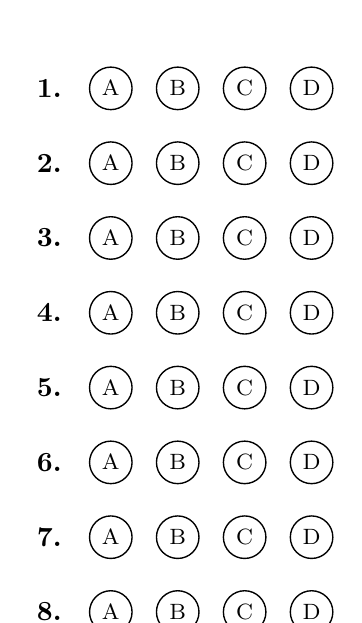
\begin{tikzpicture}[x=1cm,y=1cm]
\node[anchor=east] at (0.55,0.00) {\textbf{1.}};
\draw[line width=0.5pt] (1.05,0.00) circle (0.27);
\node at (1.05,0.00) {\footnotesize A};
\draw[line width=0.5pt] (1.90,0.00) circle (0.27);
\node at (1.90,0.00) {\footnotesize B};
\draw[line width=0.5pt] (2.75,0.00) circle (0.27);
\node at (2.75,0.00) {\footnotesize C};
\draw[line width=0.5pt] (3.60,0.00) circle (0.27);
\node at (3.60,0.00) {\footnotesize D};
\node[anchor=east] at (0.55,-0.95) {\textbf{2.}};
\draw[line width=0.5pt] (1.05,-0.95) circle (0.27);
\node at (1.05,-0.95) {\footnotesize A};
\draw[line width=0.5pt] (1.90,-0.95) circle (0.27);
\node at (1.90,-0.95) {\footnotesize B};
\draw[line width=0.5pt] (2.75,-0.95) circle (0.27);
\node at (2.75,-0.95) {\footnotesize C};
\draw[line width=0.5pt] (3.60,-0.95) circle (0.27);
\node at (3.60,-0.95) {\footnotesize D};
\node[anchor=east] at (0.55,-1.90) {\textbf{3.}};
\draw[line width=0.5pt] (1.05,-1.90) circle (0.27);
\node at (1.05,-1.90) {\footnotesize A};
\draw[line width=0.5pt] (1.90,-1.90) circle (0.27);
\node at (1.90,-1.90) {\footnotesize B};
\draw[line width=0.5pt] (2.75,-1.90) circle (0.27);
\node at (2.75,-1.90) {\footnotesize C};
\draw[line width=0.5pt] (3.60,-1.90) circle (0.27);
\node at (3.60,-1.90) {\footnotesize D};
\node[anchor=east] at (0.55,-2.85) {\textbf{4.}};
\draw[line width=0.5pt] (1.05,-2.85) circle (0.27);
\node at (1.05,-2.85) {\footnotesize A};
\draw[line width=0.5pt] (1.90,-2.85) circle (0.27);
\node at (1.90,-2.85) {\footnotesize B};
\draw[line width=0.5pt] (2.75,-2.85) circle (0.27);
\node at (2.75,-2.85) {\footnotesize C};
\draw[line width=0.5pt] (3.60,-2.85) circle (0.27);
\node at (3.60,-2.85) {\footnotesize D};
\node[anchor=east] at (0.55,-3.80) {\textbf{5.}};
\draw[line width=0.5pt] (1.05,-3.80) circle (0.27);
\node at (1.05,-3.80) {\footnotesize A};
\draw[line width=0.5pt] (1.90,-3.80) circle (0.27);
\node at (1.90,-3.80) {\footnotesize B};
\draw[line width=0.5pt] (2.75,-3.80) circle (0.27);
\node at (2.75,-3.80) {\footnotesize C};
\draw[line width=0.5pt] (3.60,-3.80) circle (0.27);
\node at (3.60,-3.80) {\footnotesize D};
\node[anchor=east] at (0.55,-4.75) {\textbf{6.}};
\draw[line width=0.5pt] (1.05,-4.75) circle (0.27);
\node at (1.05,-4.75) {\footnotesize A};
\draw[line width=0.5pt] (1.90,-4.75) circle (0.27);
\node at (1.90,-4.75) {\footnotesize B};
\draw[line width=0.5pt] (2.75,-4.75) circle (0.27);
\node at (2.75,-4.75) {\footnotesize C};
\draw[line width=0.5pt] (3.60,-4.75) circle (0.27);
\node at (3.60,-4.75) {\footnotesize D};
\node[anchor=east] at (0.55,-5.70) {\textbf{7.}};
\draw[line width=0.5pt] (1.05,-5.70) circle (0.27);
\node at (1.05,-5.70) {\footnotesize A};
\draw[line width=0.5pt] (1.90,-5.70) circle (0.27);
\node at (1.90,-5.70) {\footnotesize B};
\draw[line width=0.5pt] (2.75,-5.70) circle (0.27);
\node at (2.75,-5.70) {\footnotesize C};
\draw[line width=0.5pt] (3.60,-5.70) circle (0.27);
\node at (3.60,-5.70) {\footnotesize D};
\node[anchor=east] at (0.55,-6.65) {\textbf{8.}};
\draw[line width=0.5pt] (1.05,-6.65) circle (0.27);
\node at (1.05,-6.65) {\footnotesize A};
\draw[line width=0.5pt] (1.90,-6.65) circle (0.27);
\node at (1.90,-6.65) {\footnotesize B};
\draw[line width=0.5pt] (2.75,-6.65) circle (0.27);
\node at (2.75,-6.65) {\footnotesize C};
\draw[line width=0.5pt] (3.60,-6.65) circle (0.27);
\node at (3.60,-6.65) {\footnotesize D};
\end{tikzpicture}
\end{minipage}\hfill
\begin{minipage}[t]{0.32\textwidth}\centering
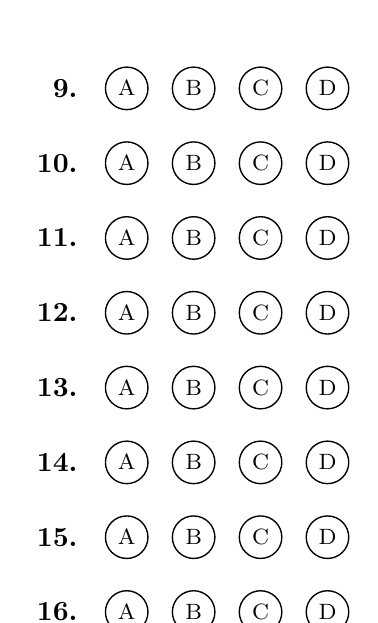
\begin{tikzpicture}[x=1cm,y=1cm]
\node[anchor=east] at (0.55,0.00) {\textbf{9.}};
\draw[line width=0.5pt] (1.05,0.00) circle (0.27);
\node at (1.05,0.00) {\footnotesize A};
\draw[line width=0.5pt] (1.90,0.00) circle (0.27);
\node at (1.90,0.00) {\footnotesize B};
\draw[line width=0.5pt] (2.75,0.00) circle (0.27);
\node at (2.75,0.00) {\footnotesize C};
\draw[line width=0.5pt] (3.60,0.00) circle (0.27);
\node at (3.60,0.00) {\footnotesize D};
\node[anchor=east] at (0.55,-0.95) {\textbf{10.}};
\draw[line width=0.5pt] (1.05,-0.95) circle (0.27);
\node at (1.05,-0.95) {\footnotesize A};
\draw[line width=0.5pt] (1.90,-0.95) circle (0.27);
\node at (1.90,-0.95) {\footnotesize B};
\draw[line width=0.5pt] (2.75,-0.95) circle (0.27);
\node at (2.75,-0.95) {\footnotesize C};
\draw[line width=0.5pt] (3.60,-0.95) circle (0.27);
\node at (3.60,-0.95) {\footnotesize D};
\node[anchor=east] at (0.55,-1.90) {\textbf{11.}};
\draw[line width=0.5pt] (1.05,-1.90) circle (0.27);
\node at (1.05,-1.90) {\footnotesize A};
\draw[line width=0.5pt] (1.90,-1.90) circle (0.27);
\node at (1.90,-1.90) {\footnotesize B};
\draw[line width=0.5pt] (2.75,-1.90) circle (0.27);
\node at (2.75,-1.90) {\footnotesize C};
\draw[line width=0.5pt] (3.60,-1.90) circle (0.27);
\node at (3.60,-1.90) {\footnotesize D};
\node[anchor=east] at (0.55,-2.85) {\textbf{12.}};
\draw[line width=0.5pt] (1.05,-2.85) circle (0.27);
\node at (1.05,-2.85) {\footnotesize A};
\draw[line width=0.5pt] (1.90,-2.85) circle (0.27);
\node at (1.90,-2.85) {\footnotesize B};
\draw[line width=0.5pt] (2.75,-2.85) circle (0.27);
\node at (2.75,-2.85) {\footnotesize C};
\draw[line width=0.5pt] (3.60,-2.85) circle (0.27);
\node at (3.60,-2.85) {\footnotesize D};
\node[anchor=east] at (0.55,-3.80) {\textbf{13.}};
\draw[line width=0.5pt] (1.05,-3.80) circle (0.27);
\node at (1.05,-3.80) {\footnotesize A};
\draw[line width=0.5pt] (1.90,-3.80) circle (0.27);
\node at (1.90,-3.80) {\footnotesize B};
\draw[line width=0.5pt] (2.75,-3.80) circle (0.27);
\node at (2.75,-3.80) {\footnotesize C};
\draw[line width=0.5pt] (3.60,-3.80) circle (0.27);
\node at (3.60,-3.80) {\footnotesize D};
\node[anchor=east] at (0.55,-4.75) {\textbf{14.}};
\draw[line width=0.5pt] (1.05,-4.75) circle (0.27);
\node at (1.05,-4.75) {\footnotesize A};
\draw[line width=0.5pt] (1.90,-4.75) circle (0.27);
\node at (1.90,-4.75) {\footnotesize B};
\draw[line width=0.5pt] (2.75,-4.75) circle (0.27);
\node at (2.75,-4.75) {\footnotesize C};
\draw[line width=0.5pt] (3.60,-4.75) circle (0.27);
\node at (3.60,-4.75) {\footnotesize D};
\node[anchor=east] at (0.55,-5.70) {\textbf{15.}};
\draw[line width=0.5pt] (1.05,-5.70) circle (0.27);
\node at (1.05,-5.70) {\footnotesize A};
\draw[line width=0.5pt] (1.90,-5.70) circle (0.27);
\node at (1.90,-5.70) {\footnotesize B};
\draw[line width=0.5pt] (2.75,-5.70) circle (0.27);
\node at (2.75,-5.70) {\footnotesize C};
\draw[line width=0.5pt] (3.60,-5.70) circle (0.27);
\node at (3.60,-5.70) {\footnotesize D};
\node[anchor=east] at (0.55,-6.65) {\textbf{16.}};
\draw[line width=0.5pt] (1.05,-6.65) circle (0.27);
\node at (1.05,-6.65) {\footnotesize A};
\draw[line width=0.5pt] (1.90,-6.65) circle (0.27);
\node at (1.90,-6.65) {\footnotesize B};
\draw[line width=0.5pt] (2.75,-6.65) circle (0.27);
\node at (2.75,-6.65) {\footnotesize C};
\draw[line width=0.5pt] (3.60,-6.65) circle (0.27);
\node at (3.60,-6.65) {\footnotesize D};
\end{tikzpicture}
\end{minipage}\hfill
\begin{minipage}[t]{0.32\textwidth}\centering
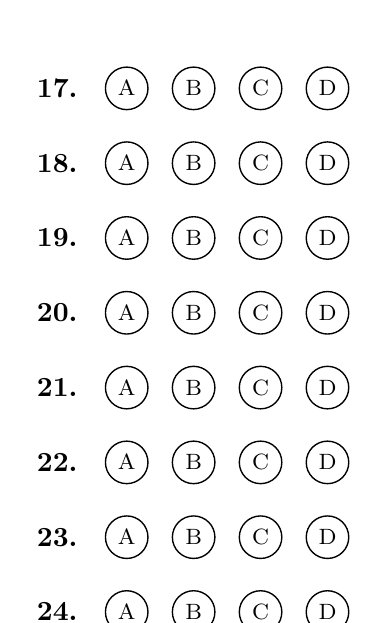
\begin{tikzpicture}[x=1cm,y=1cm]
\node[anchor=east] at (0.55,0.00) {\textbf{17.}};
\draw[line width=0.5pt] (1.05,0.00) circle (0.27);
\node at (1.05,0.00) {\footnotesize A};
\draw[line width=0.5pt] (1.90,0.00) circle (0.27);
\node at (1.90,0.00) {\footnotesize B};
\draw[line width=0.5pt] (2.75,0.00) circle (0.27);
\node at (2.75,0.00) {\footnotesize C};
\draw[line width=0.5pt] (3.60,0.00) circle (0.27);
\node at (3.60,0.00) {\footnotesize D};
\node[anchor=east] at (0.55,-0.95) {\textbf{18.}};
\draw[line width=0.5pt] (1.05,-0.95) circle (0.27);
\node at (1.05,-0.95) {\footnotesize A};
\draw[line width=0.5pt] (1.90,-0.95) circle (0.27);
\node at (1.90,-0.95) {\footnotesize B};
\draw[line width=0.5pt] (2.75,-0.95) circle (0.27);
\node at (2.75,-0.95) {\footnotesize C};
\draw[line width=0.5pt] (3.60,-0.95) circle (0.27);
\node at (3.60,-0.95) {\footnotesize D};
\node[anchor=east] at (0.55,-1.90) {\textbf{19.}};
\draw[line width=0.5pt] (1.05,-1.90) circle (0.27);
\node at (1.05,-1.90) {\footnotesize A};
\draw[line width=0.5pt] (1.90,-1.90) circle (0.27);
\node at (1.90,-1.90) {\footnotesize B};
\draw[line width=0.5pt] (2.75,-1.90) circle (0.27);
\node at (2.75,-1.90) {\footnotesize C};
\draw[line width=0.5pt] (3.60,-1.90) circle (0.27);
\node at (3.60,-1.90) {\footnotesize D};
\node[anchor=east] at (0.55,-2.85) {\textbf{20.}};
\draw[line width=0.5pt] (1.05,-2.85) circle (0.27);
\node at (1.05,-2.85) {\footnotesize A};
\draw[line width=0.5pt] (1.90,-2.85) circle (0.27);
\node at (1.90,-2.85) {\footnotesize B};
\draw[line width=0.5pt] (2.75,-2.85) circle (0.27);
\node at (2.75,-2.85) {\footnotesize C};
\draw[line width=0.5pt] (3.60,-2.85) circle (0.27);
\node at (3.60,-2.85) {\footnotesize D};
\node[anchor=east] at (0.55,-3.80) {\textbf{21.}};
\draw[line width=0.5pt] (1.05,-3.80) circle (0.27);
\node at (1.05,-3.80) {\footnotesize A};
\draw[line width=0.5pt] (1.90,-3.80) circle (0.27);
\node at (1.90,-3.80) {\footnotesize B};
\draw[line width=0.5pt] (2.75,-3.80) circle (0.27);
\node at (2.75,-3.80) {\footnotesize C};
\draw[line width=0.5pt] (3.60,-3.80) circle (0.27);
\node at (3.60,-3.80) {\footnotesize D};
\node[anchor=east] at (0.55,-4.75) {\textbf{22.}};
\draw[line width=0.5pt] (1.05,-4.75) circle (0.27);
\node at (1.05,-4.75) {\footnotesize A};
\draw[line width=0.5pt] (1.90,-4.75) circle (0.27);
\node at (1.90,-4.75) {\footnotesize B};
\draw[line width=0.5pt] (2.75,-4.75) circle (0.27);
\node at (2.75,-4.75) {\footnotesize C};
\draw[line width=0.5pt] (3.60,-4.75) circle (0.27);
\node at (3.60,-4.75) {\footnotesize D};
\node[anchor=east] at (0.55,-5.70) {\textbf{23.}};
\draw[line width=0.5pt] (1.05,-5.70) circle (0.27);
\node at (1.05,-5.70) {\footnotesize A};
\draw[line width=0.5pt] (1.90,-5.70) circle (0.27);
\node at (1.90,-5.70) {\footnotesize B};
\draw[line width=0.5pt] (2.75,-5.70) circle (0.27);
\node at (2.75,-5.70) {\footnotesize C};
\draw[line width=0.5pt] (3.60,-5.70) circle (0.27);
\node at (3.60,-5.70) {\footnotesize D};
\node[anchor=east] at (0.55,-6.65) {\textbf{24.}};
\draw[line width=0.5pt] (1.05,-6.65) circle (0.27);
\node at (1.05,-6.65) {\footnotesize A};
\draw[line width=0.5pt] (1.90,-6.65) circle (0.27);
\node at (1.90,-6.65) {\footnotesize B};
\draw[line width=0.5pt] (2.75,-6.65) circle (0.27);
\node at (2.75,-6.65) {\footnotesize C};
\draw[line width=0.5pt] (3.60,-6.65) circle (0.27);
\node at (3.60,-6.65) {\footnotesize D};
\end{tikzpicture}
\end{minipage}\hfill

\vspace{3em}
\begin{center}
\large Score \quad \underline{\hspace{2cm}} \,/\, 24
\end{center}


\newpage
\begin{center}
  {\Large\bfseries Formula Sheet}\\[3pt]
  {\small\itshape Use this page only if your exam provides a formula sheet.}\\[2pt]
  \rule{\textwidth}{0.4pt}
\end{center}

\subsection*{Fitness}
\begin{center}\renewcommand{\arraystretch}{2.1}
\begin{tabular}{r@{\;}l@{\qquad}l}
  \(w\) & \(=\ \text{viability} \times \text{fecundity}\) & absolute fitness, offspring left per zygote\\
  \(W\) & \(=\ w / w_{\max}\) & relative fitness\\
  \(s\) & \(=\ 1 - W\) & selection coefficient
\end{tabular}\end{center}

\subsection*{Mean fitness and the general equation}
\begin{align*}
  \overline{W} &= f(AA)\,W_{AA} + f(Aa)\,W_{Aa} + f(aa)\,W_{aa}\\[4pt]
  q' &= \frac{\tfrac{1}{2}\,f(Aa)\,W_{Aa} + f(aa)\,W_{aa}}{\overline{W}}, \qquad \Delta q = q' - q
\end{align*}
Under Hardy--Weinberg, \(f(AA)=p^2\), \(f(Aa)=2pq\), \(f(aa)=q^2\). With counted individuals that selection acts on directly, use the counted frequencies.

\subsection*{Average excess}
\begin{align*}
  \alpha_a &= q\,W_{aa} + p\,W_{Aa} - \overline{W}, & \Delta q &= \frac{q}{\overline{W}}\,\alpha_a\\[4pt]
  \alpha_A &= p\,W_{AA} + q\,W_{Aa} - \overline{W}, & \Delta p &= \frac{p}{\overline{W}}\,\alpha_A
\end{align*}
Requires Hardy--Weinberg genotype frequencies.

\subsection*{Special models (\(q\) is always the allele selected against)}
\begin{align*}
  \text{Against the recessive:}\quad \Delta q &= \frac{-s\,p\,q^2}{1 - s\,q^2}\\[4pt]
  \text{Against the dominant:}\quad \Delta q &= \frac{-s\,p^2 q}{1 - 2sq + sq^2}
\end{align*}

\subsection*{Heterozygote advantage or disadvantage}
\[
  \hat{q} = \frac{s_1}{s_1 + s_2}
\]
with \(s_1\) for the \(p\) homozygote and \(s_2\) for the \(q\) homozygote. The equilibrium is stable under heterozygote advantage and unstable under heterozygote disadvantage.

\label{LastPage}
\end{document}